\chapter{Related Work}
\label{sec:related}
In this section, we describe a well-known theory in image enhancement.
Next, we introduce the conventional methods that apply this theory to the optimization equations with the cost functions. Finally, we consider various problems in the methods.
%----Retinex理論の説明---- %
\section{Retinex Theory} \label{sec:retinex}
The Retinex theory \cite{retinex} is a color perception model based on human visual system. The model decomposes an observed image into reflectance and illumination as follows:
\begin{equation}
S = R \circ I, \label{eq:retinex}
\end{equation}
where $S$ is an observed image, $R$ and $I$ represent reflectance and illumination, respectively. The operator $"\circ"$ denotes the element-wise multiplication. As shown in Fig.\ref{fig:retinex}, reflectance represents the intrinsic characteristics of the object and contains rich textures details. On the contrary, illumination represents the extrinsic property and contains the structure information.
%----Retinex理論のイメージ図---- %
\begin{figure}[tb]
	\begin{minipage}[b]{0.32\hsize}
		\centering
		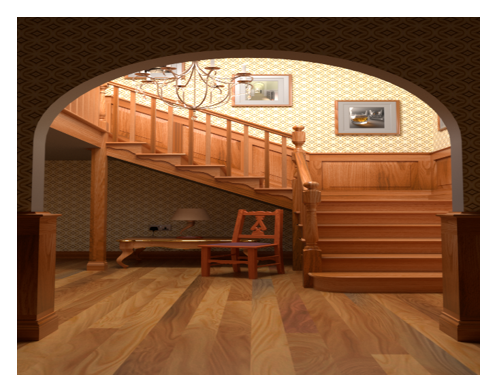
\includegraphics[height=0.75\hsize]{images/retinex/input.eps}
		\subcaption{Observed image $S$} \label{fig:reinex/input}
	\end{minipage}
	\begin{minipage}[b]{0.32\hsize}
		\centering
		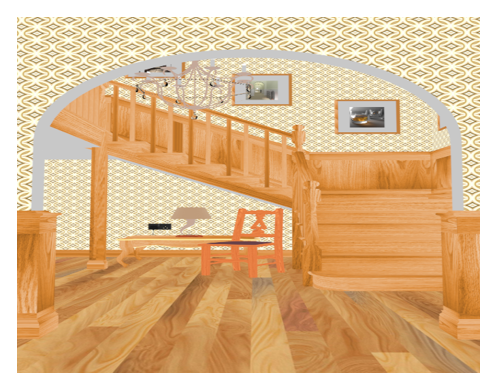
\includegraphics[height=0.75\hsize]{images/retinex/reflectance.eps}
		\subcaption{Reflectance $R$} \label{fig:retinex/reflectance}
	\end{minipage}
	\begin{minipage}[b]{0.32\hsize}
		\centering
		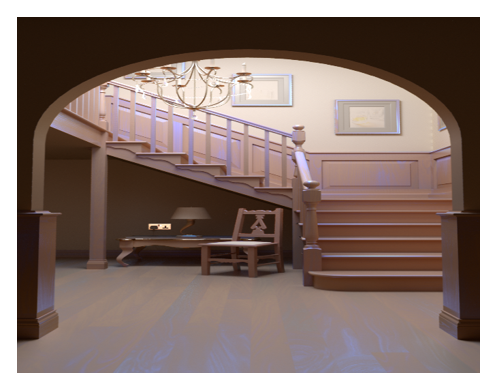
\includegraphics[height=0.75\hsize]{images/retinex/illumination.eps}
		\subcaption{Illumination $I$} \label{fig:retinex/illumination}
	\end{minipage}
\caption{The images based on the Retinex theory \cite{arpr}.}
\label{fig:retinex}
\end{figure}
The conventional Retinex-based enhancement methods such as \cite{ssr}, \cite{msr} are defined as
\begin{equation}
\log{R} = \log{S} - \log{[G \ast S]}, \label{eq:log_retinex}
\end{equation}
where $"\ast"$ represents the convolution operator, and $G$ is the Gaussian low-pass filter. This method assumes that illumination can be estimated by passing an observed image through the Gaussian low-pass filtered version of the image. Moreover, reflectance is computed by subtracting the estimated illumination from an observed image. However, this method generates halo artifacts around the edges of object when the size of the Gaussian low-pass filter is not appropriate. In addition, as shown in Fig.\ref{fig:msr}, this method causes over-enhancement and much noise in the estimated reflectance. 
\begin{figure}[tb]
\begin{minipage}[b]{0.5\hsize}
		\centering
		\includegraphics[height=0.6\hsize]{images/msr/input.eps}
		\subcaption{Observed image $S$} \label{fig:msr/input}
	\end{minipage}
	\begin{minipage}[b]{0.5\hsize}
		\centering
		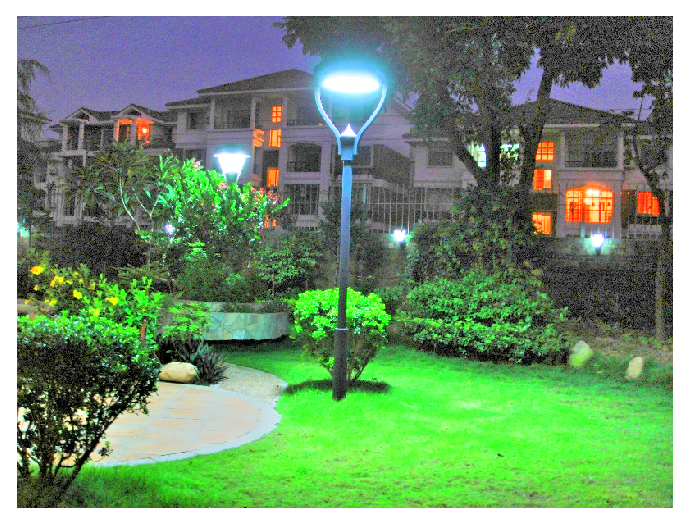
\includegraphics[height=0.6\hsize]{images/msr/reflectance.eps}
		\subcaption{Reflectance $R$} \label{fig:msr/reflectance}
	\end{minipage}
\caption{The results of the conventional Retinex-based enhancement method \cite{msr}.}
\label{fig:msr}
\end{figure}

%----Variational Retinex Modelの説明---- %
\section{Variational Retinex Model} \label{sec:variational_retinex}
Various methods have proposed optimization problems based on the Retinex theory in order to estimate reflectance and illumination efficiently. The methods introduce constraint terms on reflectance and illumination which consider the characteristics for them into the optimization problems. The methods usually adopt $L_{1}$ and $L_{2}$ norms to the constraint terms. For example, Fu \cite{srie} proposed the following cost function which minimizes the optimization problem:
\begin{equation}
\begin{split}
& \argmin_{R, I}{\: E(R, I)}\\ 
& E(I, R) = \|R \circ I - S\|_{2}^{2} + \alpha\|\nabla{I}\|_{2}^{2} + \beta\|\nabla{R}\|_{1} + \gamma\|I - I_{0}\|_{2}^{2} \\
& s.t. \ \ S \leqq I, \label{eq:srie_equation}
\end{split}
\end{equation}
where $\alpha$, $\beta$, $\gamma$ are three positive parameters, and $I_{0}$ is the enhanced illumination using gamma correction.
The first term $\|R \circ I - S\|_{2}^{2}$, which corresponds to L2 data fidelity, is to minimize the distance between the estimated ($R\circ{I}$) and an observed image $S$. The second term $\|\nabla{I}\|_{2}^{2} $ enforces spatially smoothness on the illumination $I$. The third term $\|\nabla{R}\|_{1}$, which corresponds to TV reflectance sparsity, enforces piece-wise continuous on the reflectance $R$. The last term $\|I-I_{0}\|_{2}^{2}$, which penalizes the brightness of illumination component, is used to avoid a scaling problem.\par
This method was implemented with a linear domain. As a result, this method can preserve more naturalness than the methods implemented with a log-transformed domain. As shown in Fig.\ref{fig:variational/srie}, this method employs the fourth term which minimizes the difference between $I$ and $I_{0}$ for the sake of suppression of over-enhancement in the estimated reflectance. Moreover, this method can suppress noise amplification due to the $L_{1}$ norm constraint term on reflectance in the estimated reflectance.
%----SRIEの図---- %
\begin{figure}[tb]
	\begin{minipage}[b]{0.5\hsize}
		\centering
		\includegraphics[width=62.5mm]{images/variational/input.eps}
		\subcaption{Observed image $S$} \label{fig:variational/input}
	\end{minipage}
	\begin{minipage}[b]{0.5\hsize}
		\centering
		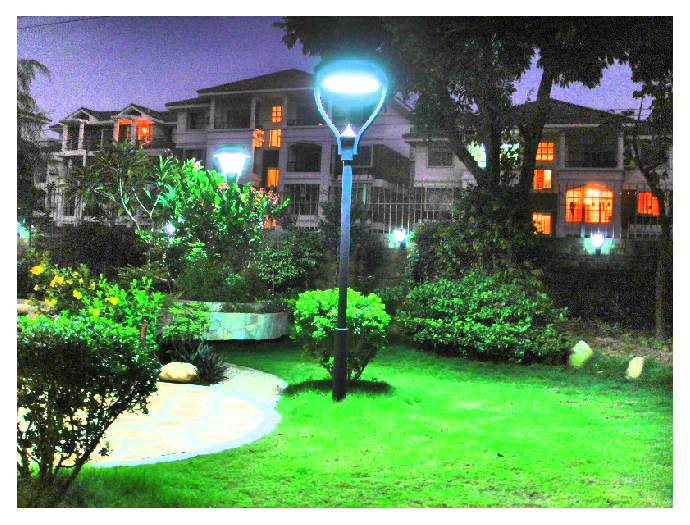
\includegraphics[width=62.5mm]{images/variational/reflectance.eps}
		\subcaption{Reflectance $R$} \label{fig:variational/reflectance}
	\end{minipage}
	\begin{minipage}[b]{0.5\hsize}
		\centering
		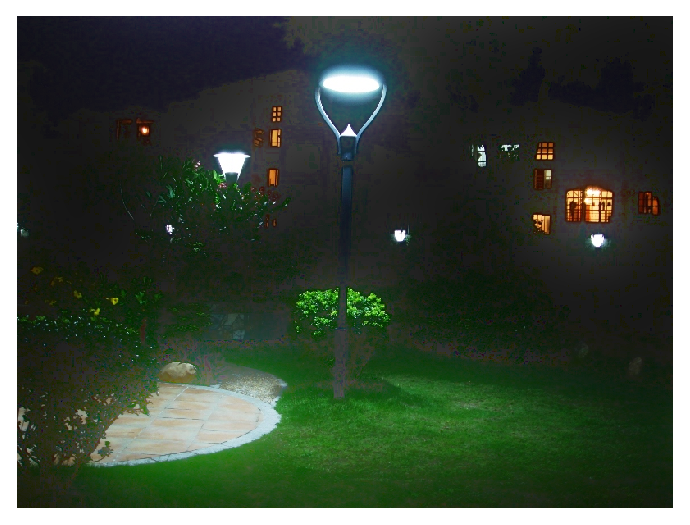
\includegraphics[width=62.5mm]{images/variational/illumination.eps}
		\subcaption{Illumination $I$} \label{fig:variational/illumination}
	\end{minipage}
	\begin{minipage}[b]{0.5\hsize}
		\centering
		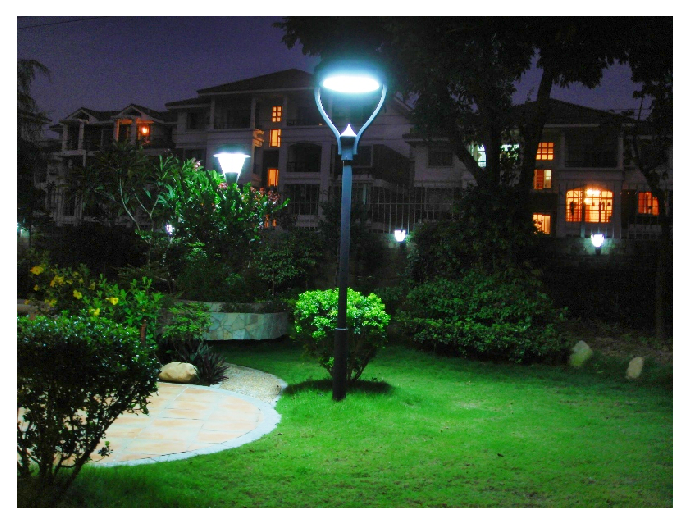
\includegraphics[width=62.5mm]{images/variational/output.eps}
		\subcaption{Enhanced image $\hat{S}$} \label{fig:variational/output}
	\end{minipage}
	\caption{The results of SRIE \cite{srie}.}
	\label{fig:variational/srie}
\end{figure}

%----Edge Preserving Filterの説明---- %
\section{Local Variation Deviation} \label{sec:lvd}
This section discusses edge/structure preserving image smoothing and a joint intrinsic-extrinsic prior model (JieP) which are proposed by Cai \cite{jiep}. This model adopted the image smoothing function as the constraint term on illumination in Eq.$(\ref{eq:srie_equation})$. 
%The illumination is piece-wisely smooth component, which can be decomposed by a edge preserving smoothing.
\par
In statics, the standard deviation represents a measure to quantify the consistency of a set of data. The local variation deviation (LVD) is used to identify different type of the variation with the statistical property. By using the feature in terms of image analysis, the LVD can surprisingly distinguish between texture and structure regions, since texture component includes weak correlation and structure component includes strong correlation. \par
The $\mathcal{R}_{d}$ denotes a relative LVD extracted from $I$:
\begin{equation}
\mathcal{R}_{d} = \left |\frac{\nabla_{d}{I}}{\frac{1}{|\Omega|}\Sigma_{\Omega}\nabla_{d}{I}+\epsilon} \right| ,
\label{eq:lvd}
\end{equation} 
where $\nabla_{d}$ is the horizontal and vertical ($d \in {h, v}$) gradient operator, $\Omega$ is the local patch size $(r \times r)$, and $\epsilon$ is a small number to avoid division by zero. 
The edge/structure preserving smoothing property of the LVD can be explained intuitively as follows:
(In the following, the mean local variation means $\bar{\nabla{I}}= \frac{1}{|\Omega|} \Sigma_{\Omega}\nabla{I}$):
\begin{itemize}
\item Case1: \textbf{Flat.} If the value of the patch $I$ is almost constant, $\nabla{I} \approx 0$ and $\bar{\nabla{I}} \approx 0$ $\rightarrow$ $\bar{\mathcal{R}} \approx 0$. 
\item Case2: \textbf{Texture.} If the value of the patch $I$ changes frequently, $\nabla{I} $ varies more rapidly than $\bar{\nabla{I}}$ $\rightarrow$ $\bar{\mathcal{R}}$ $\gg 1$.
\item Case3: \textbf{Structure.} If the value of the patch $I$ changes in accordance with structure, the deviation of $\nabla{I}$ fluctuates small $\rightarrow$ $\bar{\mathcal{R}}$ $\approx 1$.
\end{itemize}
To quantitatively analyze the effectiveness of the distinction of the LVD measure, we evaluated the average values of the LVD in the local patches in both texture and structure regions. Fig.\ref{fig:jiep/analysis} summarizes the result of this analysis. The blue squares represent texture regions and the green squares represent structure regions. We can see that there is a clear difference between texture and structure regions.
\begin{figure}[tb]
	\centering
	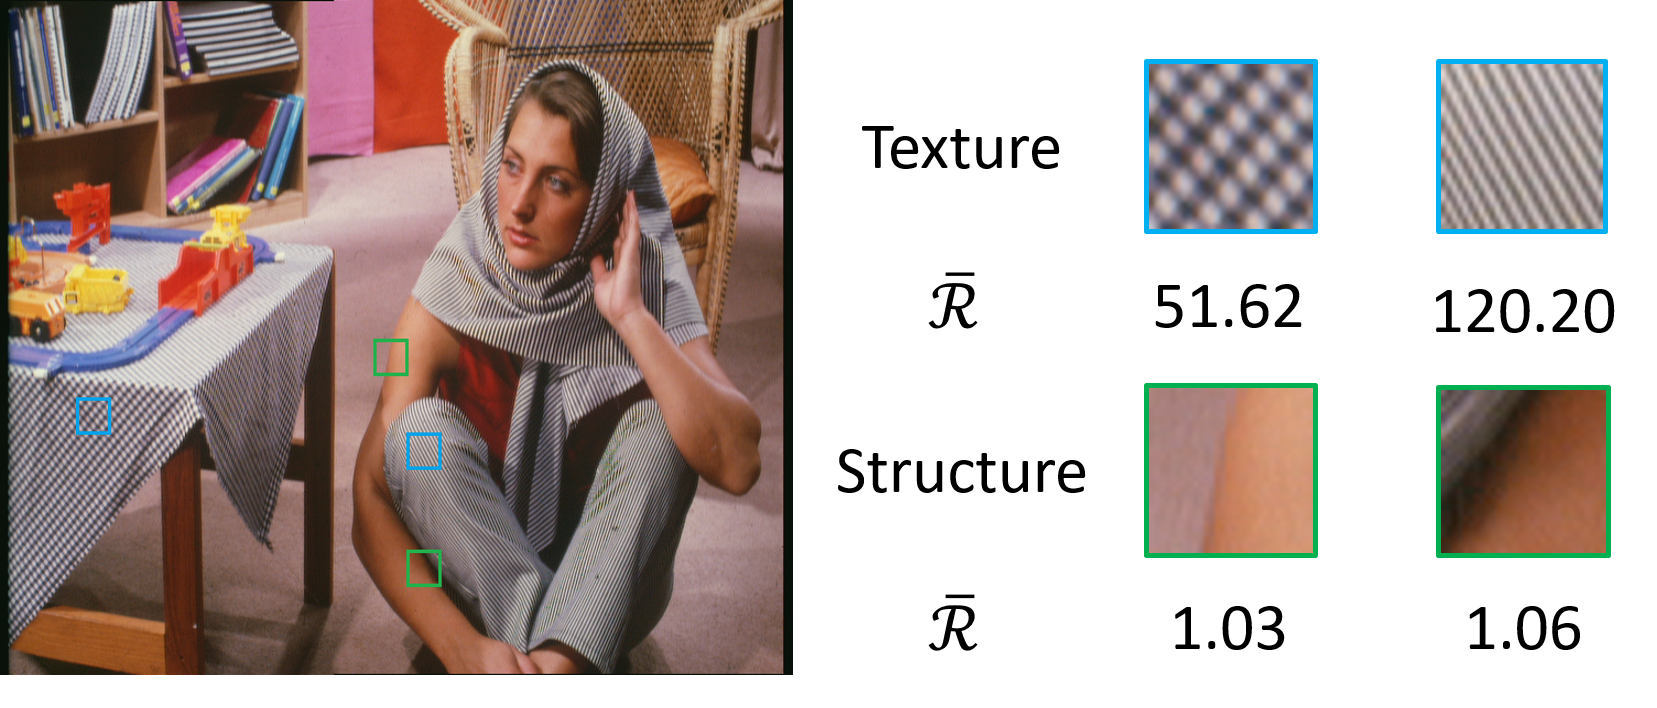
\includegraphics[width=0.8\hsize]{images/jiep/analysis/analysis.eps}
	\caption{The analysis of the local variation deviation for different patches. $\bar{\mathcal{R}}$ is the average of variation deviation in the local patches. The local variation deviation surprisingly distinguish textures (blue squares) and structures (green squares).
	} \label{fig:jiep/analysis}
\end{figure}
In order to take the effectiveness of the LVD into consideration, Cai replaced the constraint term on illumination by a $L_{1}$ norm constraint term of the LVD in a cost function to minimize an optimization problem. The function is formulated as follows:
\begin{equation}
E(I, R) = \|R \circ I - S\|_{2}^{2} + \alpha{\left \|\frac{\nabla{I}}{\frac{1}{\Omega}\Sigma_{\Omega}\nabla{I} + \epsilon} \right\|_{1}} + \beta{\|\nabla{R}\|_{1}} + \gamma{\|I - B\|_{2}^{2}}, \label{eq:jiep}
\end{equation}
where $\alpha$, $\beta$, $\gamma$ are three positive parameters and $B$ ($B = max_{\Omega}(max_{c \in \{r, g, b\}}S_{c})$) represents the bright channel prior (BCP) of an observed image $S$. As shown in Fig.\ref{fig:jiep/example}, the estimated illumination removes texture component while preserving the structure information. Thus, in the estimated reflectance, JieP significantly suppresses the awareness of halo artifacts along with edge regions. Moreover, more textures details are revealed in the estimated reflectance.
%----JiePの図---- %
\begin{figure}[tb]
	\begin{minipage}[b]{0.5\hsize}
		\centering
		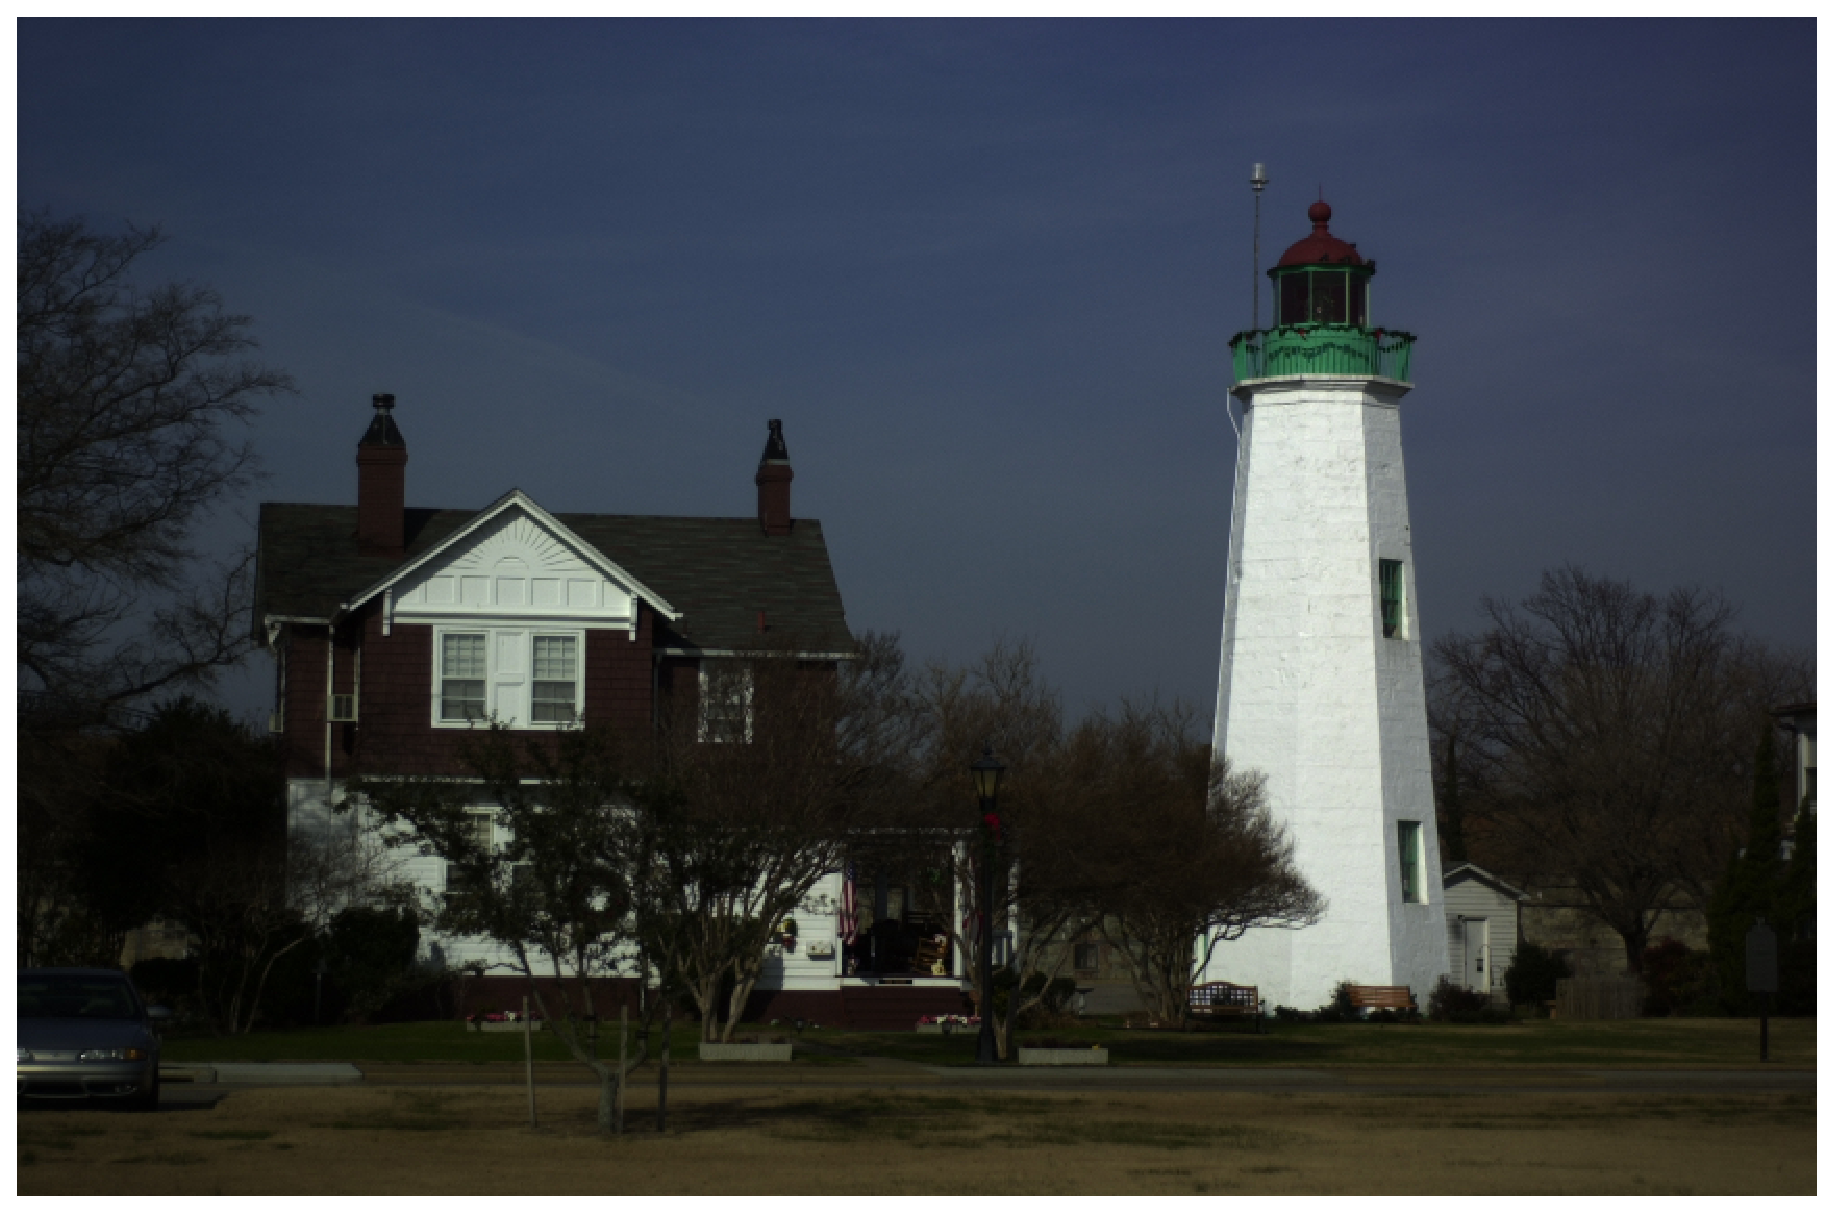
\includegraphics[width=62.5mm]{images/jiep/input.eps}
		\subcaption{Observed image $S$} \label{fig:jiep/input}
	\end{minipage}
	\begin{minipage}[b]{0.5\hsize}
		\centering
		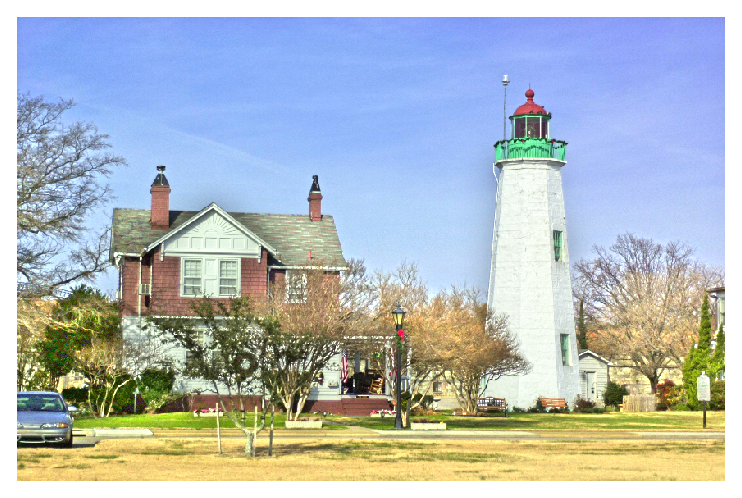
\includegraphics[width=62.5mm]{images/jiep/reflectance.eps}
		\subcaption{Reflectance $R$} \label{fig:jiep/reflectance}
	\end{minipage}
	\begin{minipage}[b]{0.5\hsize}
		\centering
		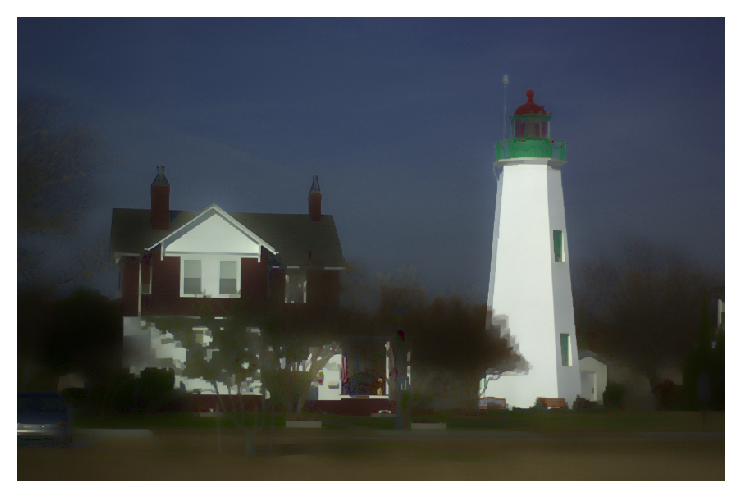
\includegraphics[width=62.5mm]{images/jiep/illumination.eps}
		\subcaption{Illumination $I$} \label{fig:jiep/illumination}
	\end{minipage}
	\begin{minipage}[b]{0.5\hsize}
		\centering
		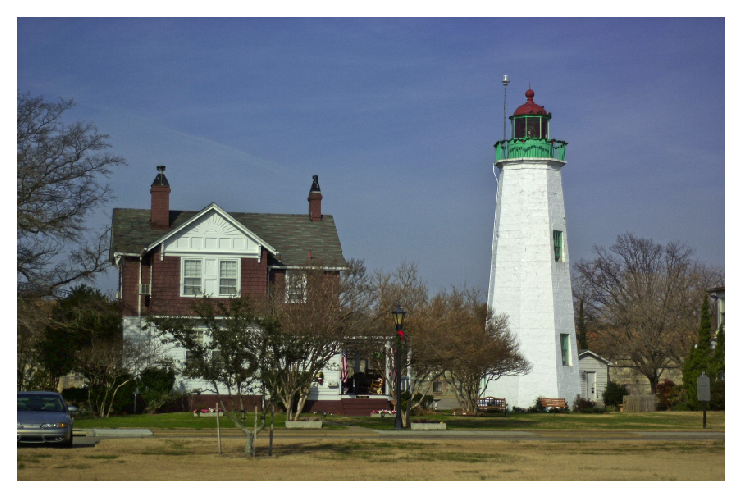
\includegraphics[width=62.5mm]{images/jiep/output.eps}
		\subcaption{Enhanced image $\hat{S}$} \label{fig:jiep/output}
	\end{minipage}
	\caption{The results of JieP \cite{jiep}.}
	\label{fig:jiep/example}
\end{figure}

\section{Consideration of Problems} \label{sec:problems}
Fu $el$ $ al.$ and Cai $et$ $al.$ can enhance low-light images by solving each minimization optimization problem.
However, the methods have some problems in the enhanced image or the estimated component.
Therefore, this section discusses such problems by using Fig.\ref{fig:problems}.
\begin{itemize}
\item \textbf{SRIE} is prone to over-smooth illumination without preserving the structure information, because the $L_{2}$ constraint term is based on the assumption that illumination should be spatially smooth. 
As a result, as shown in Fig.\ref{fig:problem/srie/reflectance}, the estimated reflectance generates halo effect along with edge regions that have large intensity gradient. 
Moreover, as can be seen in Fig.\ref{fig:variational/reflectance}, in the estimated reflectance, much noise remain in dark regions and over-enhancement causes in bright regions because the constraint term on reflectance is lack of a weight to distinguish between dark and bright regions.
\end{itemize}
\begin{itemize}
\item \textbf{JieP} can significantly take consideration of the constraint term on illumination, but is not sufficient for reflectance. Therefore, as can be seen in Fig.\ref{fig:problem/jiep/reflectance}, the estimated reflectance amplifies noise in dark regions and is over-enhanced in bright regions. Moreover, the constraint term on illumination adopts the L1 norm, so that the method may damage the structure information too much in the estimated illumination.
\end{itemize}
%----Problemsの図---- %
\begin{figure}[tb]
	\begin{minipage}[b]{1.0\hsize}
		\centering
		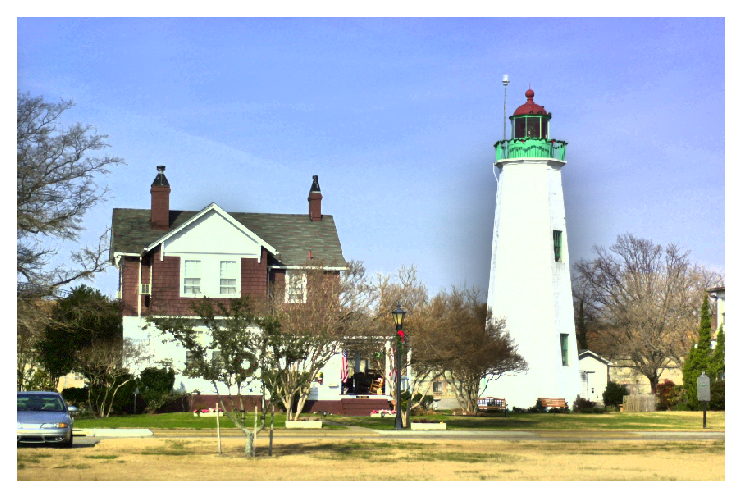
\includegraphics[width=0.65\hsize]{images/problems/srie/reflectance.eps}
		\subcaption{Reflectance (SRIE)} \label{fig:problem/srie/reflectance}
	\end{minipage}\\
	\begin{minipage}[b]{1.0\hsize}
		\centering
		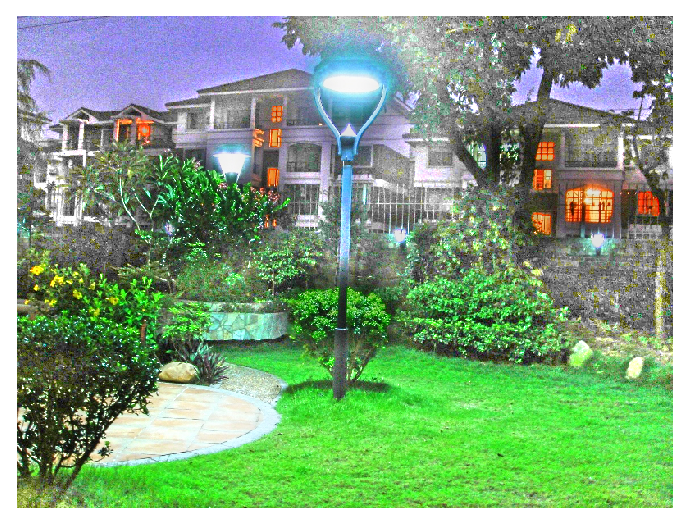
\includegraphics[width=0.65\hsize]{images/problems/jiep/reflectance.eps}
		\subcaption{Reflectance (JieP)} \label{fig:problem/jiep/reflectance}
	\end{minipage}
	\caption{Each problem which SRIE and Jiep cause in the estimated reflectance.}
	\label{fig:problems}
\end{figure}